% PARTIAL DIFFERENTIAL EQUATIONS

\section{Partial Differential Equations (PDE)}\label{sec:pde}
A partial differential equation (PDE) is defined as a differential equation that relates the derivatives
of a function such that it depends on more than one independent variable.\cite{olver_2014_pde}
This project will look at two significant classes of PDEs, namely the heat equation and the Black-Scholes equation.

\subsection{Heat Equation}\label{sec:heat}
The heat equation describes how temperature diffuses through a medium over a period of time. 
Let $u(x, \tau)$ be the temperature of a medium 
at a specific point $x$ and time $\tau$.
We denote the derivatives of $u$ with respect to $\tau\geq 0$ 
and $x\in\R$ by $u_\tau$ and $u_x$, respectively.
The heat equation \cite{leveque_2007} states that 
\begin{equation}
u_{\tau} = \kappa u_{xx}, \label{eq:heat-equation}
\end{equation}
where $\kappa$ is the thermal diffusivity constant.
The initial and boundary conditions must be defined to obtain appropriate solutions to the heat equation. 

\subsubsection{Initial and Boundary conditions over a finite interval}
For the heat equation, the initial condition is specified by
\begin{equation}
u(x,0) = u_0(x),
\end{equation}
which describes the initial temperature across the length of the medium at time $t = 0$.

Assuming that the temperature distribution falls within a finite domain, the \textit{Dirichlet} boundary conditions are applied at the extreme ends of the domain \( (0 \leq x \leq L) \), that is,
\begin{subequations}
\begin{align}
u(0,t) ={}& \alpha(t),\\
u(L,t) ={}& \beta(t).
\end{align}
\end{subequations}
For the initial and boundary conditions to be 
well posed, they need to agree at $t=0$, $x=0$, 
and $x=L$
\begin{gather*} 
\alpha(0) = u_0(0), \\
\beta(0) = u_0(L).
\end{gather*} 

\subsection{Black-Scholes Equation}\label{sec:bse}
The Black-Scholes (BS) equation is the PDE
\begin{equation}
\frac{\partial V}{\partial t} + \frac{1}{2} \sigma^2 S^2 \frac{\partial^2 V}{\partial S^2} + r S \frac{\partial V}{\partial S} - r V = 0, \label{eq:black-scholes}
\end{equation}
where \( V(S,t) \) is the price of the call/put option at time $t$ given the price of the underlying asset, $S$, 
$t$ is the time elapsed since the creation of the option, 
$r$ is the risk-free interest rate, and
$\sigma$ is the volatility of the underlying.
Based on the type of option, the BS equation is accompanied by certain terminal and boundary conditions.

\subsubsection{European Call Option}
For European call options, we use the lower boundary condition (at $S=0$)
\begin{equation}
        C(0,t) = 0, 
\end{equation}
which means that the value of option for a zero-value underlying is zero. The call option is
therefore worthless. An ``upper'' boundary condition is also imposed (at $S \rightarrow  \infty$).
This enforces that for ``very expensive'' underlying assets, the option should be priced at the same value as the underlying. 
In other words, $C(S,t) \sim S$ as $S \to  \infty$.
Practically, this condition can be imposed at a sufficiently
large value $S_{\rm max}$. A typical choice \cite{kwok_2008_derivatives} is 
\begin{equation}
        C(S_{max},t) = S_{\rm max} - Ke^{-rT}.
\end{equation}
The term $Ke^{-rT}$ represents the present value of the strike price discounted by the the risk-free
rate $r$ over the time to expiry $T$. Lastly, we impose the terminal condition (at $t = T$),
which is 
\begin{equation}
 C(S,T) = \max(S-K,0)  \label{eq:call-terminal} 
\end{equation}
for all $S$.
The option payoff $C(S,T)$ is specified at expiration $T$,
where $S$ represents the current price of the asset and $K$ denotes the strike price.

\subsubsection{European Put Option}
The case of European put options follows a different set of terminal and boundary conditions. Given the underlying asset
value at zero, the payoff becomes approximately $K$ when the option is exercised. Hence, we have
the lower boundary condition
\begin{equation}
    P(0,t) = Ke^{-rT}.
\end{equation}
On one hand, as the underlying asset $S$ becomes very large, the put option becomes inherently worthless which gives 
the upper boundary condition ($S \to \infty$)
\begin{equation}
    P(S,t) \to 0. 
\end{equation}
The terminal condition for the put option is set to
\begin{equation}
    P(S,T) = \max(K-S,0)
\end{equation}

\subsection{Equivalence between the heat equation and the Black-Scholes equation}\label{sec:equivalence} 
Following a change in variables, the Black-Scholes equation can be transformed into the one-dimensional heat equation \cite{wilmott_1995_mathematics}. Recall that the Black-Scholes equation takes the form of Equation \eqref{eq:black-scholes}.
In this analysis, we consider the case of a \textit{European call} option as an example. Here, the following substitutions can be applied to remove the $S$ term from the equation.
\begin{align} 
t ={}& T - \frac{2}{\sigma^2} \tau  \label{eq:t-substituion} \\ 
S ={}& Ke^x                         \label{eq:s-substition}  \\
V ={}& Kv(x,\tau)                   \label{eq:v-substitution}
\end{align} 
The derivatives can now be rewritten as follows
\begin{align}
    V_t 
{}={}& 
    \frac{\partial V}{\partial t} 
    {}={} 
    \frac{\partial V}{\partial \tau} \frac{d \tau}{dt} 
    {}={} 
    -\frac{\sigma^2}{2} \frac{dV}{d\tau} 
    {}={}  -\frac{1}{2} \sigma^2 V_{\tau}
\\
    V_S
{}={}& 
    \frac{\partial V}{\partial S} 
    {}={} 
    \frac{\partial V}{\partial x} \frac{dx}{dS} 
    {}={} 
    \frac{1}{S} \frac{\partial V}{\partial x} 
    {}={}
    \frac{1}{S} V_x
\\
    V_{SS} 
{}={}& 
    \frac{\partial^2 V}{\partial S^2} 
    {}={} 
    \frac{\partial V_S}{\partial S} 
\notag\\
{}={}& 
    \frac{\partial}{\partial S} \left( \frac{1}{S} \frac{\partial V}{\partial x} \right) 
\notag\\
{}={}& 
    -\frac{1}{S^2} \frac{\partial V}{\partial x} + \frac{1}{S} \frac{\partial V}{\partial x} \frac{\partial V}{\partial x} \frac{dx}{\partial S} 
\notag\\
{}={}& 
    -\frac{1}{S^2} V_x + \frac{1}{S} V_{xx} \frac{1}{S} 
\notag\\
{}={}& 
    -\frac{1}{S^2} V_x + \frac{1}{S^2} V_{xx},
\end{align}
which leads to the following form of the equation
\begin{equation}
\begin{aligned}
& V_t + \frac{1}{2}\sigma^2 S^2 V_{SS} + rSV_S - rV =  0
\\
\Rightarrow{}&{}  -\frac{1}{2}\sigma^2 V_{\tau} + \frac{1}{2} \sigma^2 (V_{xx} - V_x) + rV_x - rV = 0
\\
\Rightarrow{}&{} -\frac{1}{2}\sigma^2 V_{\tau} + \frac{1}{2} \sigma^2 V_{xx} -\frac{1}{2}\sigma^2 V_x + rV_x - rV = 0
\\
\Rightarrow{}&{} -\frac{1}{2}\sigma^2 V_{\tau} + \frac{1}{2} \sigma^2 V_{xx} + (r - \frac{1}{2}\sigma^2)V_x - rV = 0,
\end{aligned}
\end{equation}
where it can be further simplified by dividing 
by $-\frac{1}{2}\sigma^2$ to yield
\begin{equation}
    V_{\tau} - V_{xx} + (1-\lambda)V_x + \lambda V = 0, \label{eq:V_simplified}
\end{equation}
where $\lambda = \frac{2r}{\sigma^2}$. The initial condition for this equation comes from the payoff of the option at $\tau = 0$. For a call option, the payoff
is described by \eqref{eq:call-terminal}. Using the substitution from \eqref{eq:s-substition}, the initial condition is
\begin{equation}
    V(Ke^x, T) = \max(Ke^x - K, 0) = K \max(e^x - 1, 0),
\end{equation}
where the K term can be factored out to give
\begin{equation}
    V(x,0) = \max(e^x - 1, 0).
\end{equation}
Now, the transformation
\begin{equation}
V(x,\tau) = e^{ax+b\tau} u(x,\tau) 
\end{equation}
is introduced to eliminate the $V$ term and its corresponding derivatives and thus convert the equation to the heat equation.
The partial derivatives of $V$ in terms of $u$ are
\begin{align}
    V_x {}={}& ae^{ax+b\tau}u(x,\tau) + e^{ax+b\tau}u_x(x,\tau) = e^{ax+b\tau}(au + u_x) \label{Vx_simplified}
    \\
    V_{\tau} {}={}& be^{ax+b\tau}u(x,\tau) + e^{ax+b\tau}u_{\tau} = e^{ax+b\tau}(bu + u_{\tau}) \label{Vtau_simplified}
    \\
    V_{xx} {}={}& ae^{ax+b\tau}(au+u_x) + e^{ax+b\tau}(au_x+u_{xx}) = e^{ax+b\tau}(u_{xx} + 2au_x + a^2u) \label{Vxx_simplified}
\end{align}
Substituting equations (\ref{Vx_simplified}), (\ref{Vxx_simplified}) , (\ref{Vtau_simplified}) into Equation (\ref{eq:V_simplified}), using $k = e^{ax+b\tau}$, yields the following:
\begin{equation}
\begin{aligned}
    & \cancel{k}(bu+u_x)-\cancel{k}(u_{xx}+2au_x+a^2u)+(1-\lambda)\cancel{k}(au+u_x)+\lambda \cancel{k}u = 0 \\
    & bu + u_x - u_{xx} - 2au_x - a^2u+(1-\lambda)au +(1-\lambda)u_x+\lambda u = 0
\end{aligned}
\end{equation}
which gives
\begin{equation}
    (b-a^2+a(1-\lambda)+\lambda)u + u_\tau - u_{xx} - (2a-(1-\lambda))u_x = 0 \label{eq:v_transformed}
\end{equation}
Note that the heat equation in \eqref{eq:heat-equation} consists only of $u_\tau$ and $u_{xx}$. 
To fully transform Equation \eqref{eq:v_transformed} to the heat equation, the terms $u_x$ and $u$ need to be eliminated by setting their coefficients to 0, which can be achieved by the substitutions
\begin{align} 
a ={}& \frac{1-\lambda}{2}, \\ 
b ={}& a^2-a(1-\lambda)-\lambda = -\frac{(\lambda+1)^2}{4}
\end{align}
Ultimately, leading to the heat equation,
\begin{equation}
    u_\tau = u_{xx}
\end{equation}
with the initial condition
\begin{equation}
    u(x,0) = \max(e^{\frac{1}{2} (\lambda + 1)x} - e^{\frac{1}{2} (\lambda - 1)x}, 0).
\end{equation}

% STOCHASTIC DIFFERENTIAL EQUATIONS

\section{Stochastic differential equations}
\newtheorem{theorem}{Theorem}[section]
\theoremstyle{definition}
\newtheorem{definition}{Definition}[section]

Stochastic differential equations play an integral role in the mathematical modelling of financial processes, particularly due 
to their ability to capture the uncertainty and randomness that is inherent in financial markets. A \textit{stochastic process} is defined as a collection of random variables indexed by time,
where each variable represents the state of the system at a given time.

\subsection{Brownian motion}
\begin{definition}
    The standard (one-dimensional) \textit{Brownian motion} is defined as a continous-time \textit{stochastic process} such that it satisfies the following properties:
    \begin{enumerate}[(1)]
        \item $B_0 = 0$,
        \item the paths (the function $t \rightarrow B_t(\omega)$) are continuous in $t$ a.s.,
        \item the process $\{ B_t \}_{t \geq 0}$ has stationary and independent increments,
        \item the increments $B_{t+h} - B_t$ follow a normal distribution with mean 0 and variance $h$.
    \end{enumerate}
\end{definition}

The third property of the standard \textit{Brownian motion} implies that it is a \textit{Markov process} where the future behaviour of the process
depends only on its present value and is independent of its past history.

\begin{figure}[H]
    \centering
    \includegraphics[width=0.8\textwidth]{figures/brownian_plot.pdf}
    \caption{Sample paths of a standard Brownian motion.}
    \label{fig:bm-sample-paths}
\end{figure}

\subsection{It\^{o} Integral}

When working with stochastic processes, standard Riemann integrals are not sufficient enough to capture the stochastic nature of the process. 
The non-differentiable paths of the Brownian motion demand a different approach to integration, which is where the \textit{It\^{o} integral} comes into play.

\begin{definition}
A filtration $\mathcal{F}_t$ is an increasing collection of sigma-algebras that represents the history of a stochastic process up to time $t$.
\end{definition}

\begin{definition}
An $\mathcal{F}_t$-adapted process $f_t$ is said to be elementary if it is a piece-wise constant function of the form 
\begin{equation}
    f_t(\omega) = \sum_{i} e_i(\omega) \cdot \mathbb{I}_{[t_i, t_{i+1})}(t),
\end{equation}
where there exists a series of stopping times $0 = t_0 < t_1 < \ldots < t_n = T$, and $\mathbb{I}_{[t_i, t_{i+1})} = 1$ if $t \in [t_i, t_{i+1})$ or 0 otherwise.
Note that the function $e_i(\omega)$ is $\mathcal{F}_{t_i}$ measurable and is bounded in the interval $[t_i, t_{i+1})$.
\end{definition}
\begin{definition}
    Given a stochastic process $f_t$ adapted to a filtration $\mathcal{F}_t$ and a Brownian motion $B_t$ over an interval $[0,T]$, the \textit{It\^{o} integral} of an elementary process is defined as
    \begin{equation}
        % Y_t = \int_0^t f_t(\omega) dB_t(\omega) = \lim_{n \to \infty} \sum_{i=0}^{n-1} f_{t_i}(\omega) \cdot (B_{t_{i+1}}(\omega) - B_{t_i} (\omega)),
        Y_t = \int_0^T f_t(\omega) dB_t(\omega) := \sum_{i = 0}^{n-1} e_i (\omega) \cdot (B_{t_{i+1}}(\omega) - B_{t_i} (\omega)),
    \end{equation}
    where $Y_t$ is a newly defined stochastic process based on the stochastic processes $f_t$ and $B_t$.
\end{definition}

\subsubsection{It\^{o} integral for General Integrands}
Here, the It\^{o} integral is extended to general integrands where the integrand is not necessarily elementary; Instead, we have
integrands that undergo continuous variations and jumps\cite{shreve_2004_stochastic2}.
\begin{definition}
    The \textit{It\^{o} integral} for general integrands $X_t(\omega)$ is defined as
    \begin{equation}
        \int_0^T X_t(\omega) dB_t(\omega) = \lim_{n \to \infty} \int_0^T X_{t}^{(n)}(\omega) dB_t(\omega),
    \end{equation}
    where $X_{t}^{(n)}(\omega)$ represents a sequence of elementary processes that converges to $X_t(\omega)$, i.e., in $L^2([0,T] \times \Omega).$
\end{definition}


% IMPORTANT COMMENTS
% + Some plots of paths of the BM 

% + Ito integrals: what they are (define them for elementary 
% functions, extend using the limit).
%  talk about martingale

% GBM
% + plots.
% + what are some basic properties of GBM? (lognormal distribution)
% + What do we use it for? (stock price modelling)


\subsection{It\^{o} processes}
Let $B_t$ be a 1-dimensional \textit{Brownian motion}. An \textit{It\^{o} process} is represented by the stochastic differential equation (SDE)
\begin{equation}
    dX_t = a(t, X_t) dt + \sigma(t, X_t) dB_t, \label{eq:ito-process}
\end{equation}
where $a(t, X_t)$ is known as the \textit{drift} term and $\sigma(t, X_t)$ is the diffusion term. The SDE can otherwise be rewritten in the form
\begin{equation}
    X_t = X_0 + \int_0^t a(s, X_s) dt + \int_0^t \sigma(s, X_s) dB_s.
\end{equation}
\begin{theorem}[Ito's Lemma~\cite{oksendal_2003_sde}]
    \label{thm:ito-lemma}
    Suppose $X_t$ is an It\^{o} process given by \eqref{eq:ito-process}. Let $g(t, x)$ be a function such that $g$ is twice continuously differentiable (i.e. $g \in C^2$ on $\left [ 0, \infty \right ) \times \mathbb{R}$).
    Then, the function $Y_t = g(t, X_t)$ is also an It\^{o} process where the SDE is given by
    \begin{equation}
        dY_t = \frac{\partial g}{\partial t} (t, X_t) dt + \frac{\partial g}{\partial x} (t, X_t) dX_t + \frac{1}{2} \frac{\partial^2 g}{\partial x^2} (t, X_t) \cdot (dX_t)^2,
    \end{equation}
    where $(dX_t)^2 = (dX_t) \cdot (dX_t)$ follows the It\^{o} calculus rules
    \begin{equation}
        dt \cdot dt = dt \cdot dB_t = dB_t \cdot dt = 0, \quad dB_t \cdot dB_t = dt. \label{eq:ito-calculus_rules}
    \end{equation}
\end{theorem}

\subsection{Geometric Brownian motion (GBM)}
A stochastic process $S_t$ is said to follow a \textit{Geometric Brownian motion} with drift rate $\mu$ and volatility $\sigma$ if it satisfies the SDE
\begin{equation}
    dS_t = \mu S_t dt + \sigma S_t dB_t, \label{eq:gbm}
\end{equation}
where $B_t$ is a standard Brownian motion.

\subsubsection{Solution to the GBM Stochastic Differential Equation}
Let $S_t$ be a stochastic process that satisfies \textit{Geometric Brownian motion}. By applying It\^{o}'s Lemma (Theorem \ref{thm:ito-lemma}) to the function $ Y_t = g(t, S_t) = \log S_t$, we obtain the resulting SDE for $Y_t$:
\begin{equation}
    dY_t = g_t dt + g_x dX_t + \frac{1}{2} g_{xx} (dX_t)^2,
\end{equation}
which is equivalent to
\begin{align}
    d(\log S_t) 
    {}={}& \frac{\partial \log S_t}{\partial t} dt + \frac{\partial \log S_t}{\partial t} dS_t + \frac{1}{2} \frac{\partial^2 \log S_t}{\partial S_t^2} (dS_t)^2 \notag\\
    {}={}& \frac{1}{S_t} dS_t - \frac{1}{2} (\frac{1}{{S_t}^2}) (dS_t)^2. \label{eq:ito-gbm}
\end{align}
Using the SDE in equation \eqref{eq:gbm} for $S_t$ under the assumption of GBM, we can compute the $(dS_t)^2$ term to get
\begin{equation}
    (dS_t)^2 = (\mu S_t dt + \sigma S_t dB_t)^2 = \sigma ^2 {S_t}^2 dt.
\end{equation}
Substituting this back into equation \eqref{eq:ito-gbm} leaves us with the simplified form:
\begin{equation}
    d(\log S_t) = \mu dt + \sigma dB_t - \frac{1}{2} \sigma^2 dt = (\mu - \frac{1}{2} \sigma^2) dt + \sigma dB_t. \label{eq:ito-gbm-simplified}
\end{equation}
Integrating both sides of the equation using $\beta = \mu - \frac{1}{2} \sigma^2$, the solution to the SDE is given by
\begin{equation}
    \log S_t = \log S_0 + (\mu - \frac{1}{2} \sigma^2) t + \sigma B_t, \label{eq:log-gbm}
\end{equation}
which is otherwise known as
\begin{equation}
    S_t = S_0 e^{(\beta t + \sigma B_t)}. \label{eq:gbm-solution}
\end{equation}

\subsubsection{Lognormal Property}
Here, it is observed that the solution \eqref{eq:gbm-solution} to the \textit{Geometric Brownian motion} SDE is described by a lognormal distribution. From equation \eqref{eq:ito-gbm-simplified}, 
the constant drift rate $\mu - \frac{1}{2} \sigma^2$ and volatility $\sigma$ indicate that $Y_t = \log S_t$ follows a Brownian motion with drift. This implies that the change in $\log S_t$ is normally distributed, with the distribution given by
\begin{equation}
    \log S_t \sim N[ \log S_0 + (\mu - \frac{1}{2} \sigma^2)t, \sigma^2 t].
\end{equation}

\subsubsection{Markov property}
Like the standard Brownian motion, the \textit{Geometric Brownian motion} is also a \textit{Markov process}. This means that the future behaviour of the process depends only on its present value and is independent of its past history.

\subsubsection{Uses of GBM}
Geometric Brownian motion is typically used in Mathematical Finance, particularly to model the behaviour of stock prices \cite{hull_2021_options}.

\subsubsection{Sample Plots of Geometric Brownian motion}
\begin{figure}[H]
    \centering
    \begin{subfigure}[b]{0.495\textwidth}
        \centering
        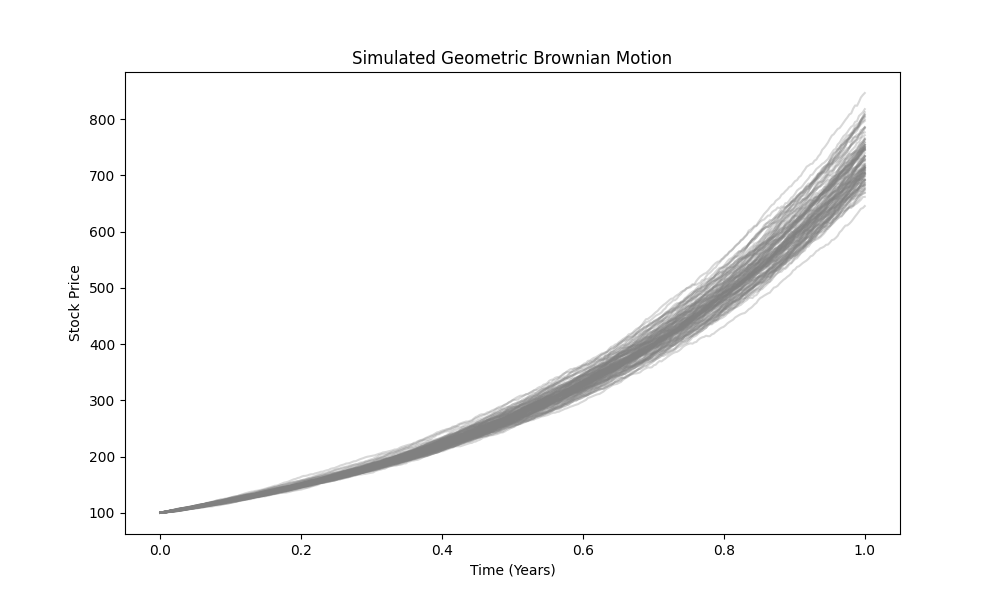
\includegraphics[width=\textwidth]{figures/gbm_plot_1.png}
        \caption{$\mu = 2, \sigma = 0.05$}
        \label{fig:gbm-sample-path-1}
    \end{subfigure}
    \hfill
    \begin{subfigure}[b]{0.495\textwidth}
        \centering
        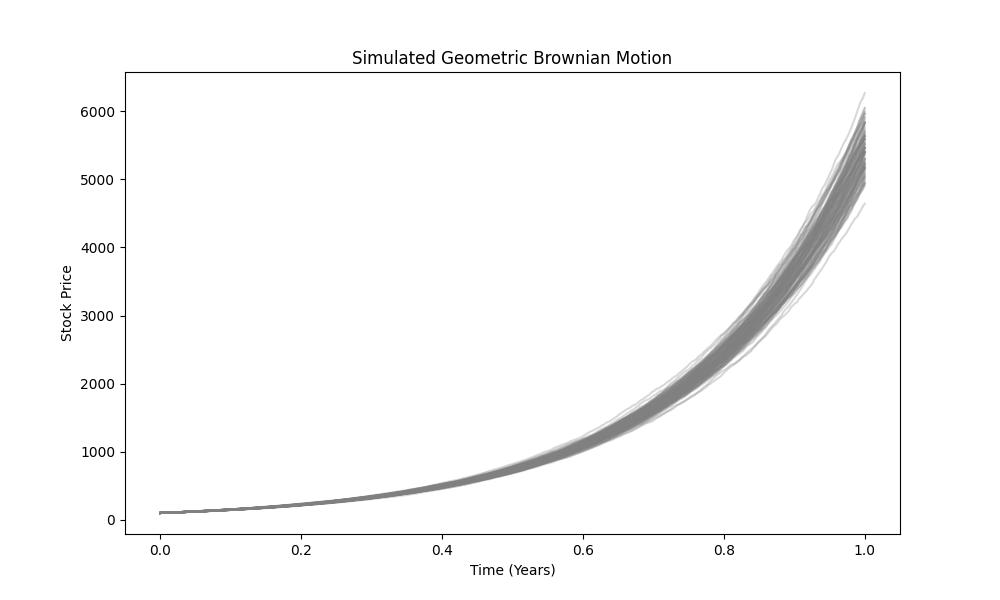
\includegraphics[width=\textwidth]{figures/gbm_plot_2.png}
        \caption{$\mu = 4, \sigma = 0.05$}
        \label{fig:gbm-sample-path-2}
    \end{subfigure}
    \begin{subfigure}[c]{0.495\textwidth}
        \centering
        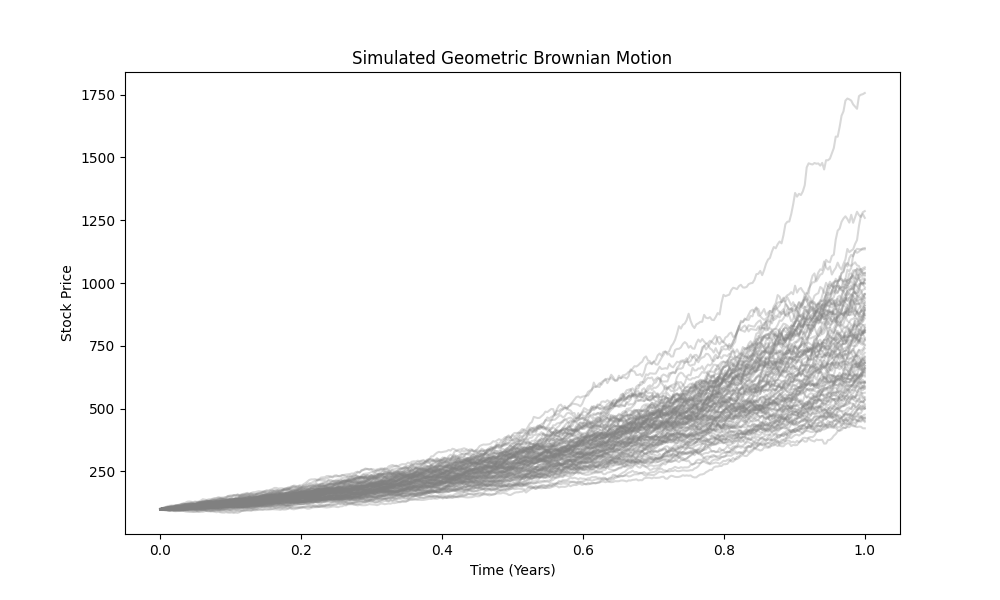
\includegraphics[width=\textwidth]{figures/gbm_plot_3.png}
        \caption{$\mu = 2, \sigma = 0.3$}
        \label{fig:gbm-sample-path-3}
    \end{subfigure}
    \caption{Sample paths of Geometric Brownian motion for different $\mu$ and $\sigma$ values.}
    \label{fig:gbm-sample-paths}
\end{figure}


\subsection{Black-Scholes Differential Equation}
The Black-Scholes PDE is derived based on a set of assumptions that model the behaviour of an ideal financial market - the assumptions are as follows:
\begin{enumerate}[(1)]
    \item The underlying asset price follows a \textit{Geometric Brownian motion}.
    \item Short selling of the asset is permitted.
    \item Trading of the asset can take place continuously.
    \item There are no transaction costs or taxes.
    \item There are no risk-free arbitrage opportunities.
    \item There are no dividends paid out by the undelying asset during the option's lifetime.
    \item The risk-free interest rate $r$ is constant and known.
\end{enumerate}

\subsubsection{Derivation of the Black-Scholes PDE via delta hedging} \label{sec:bse-derivation}
Consider an underlying asset at price $S_t$ which follows \textit{Geometric Brownian motion} with a known initial value $S_0 = S$.
We define a function $V(S,t)$ to represent the price of a derivative (e.g a European option). By It\^{o}'s Lemma (Theorem \ref{thm:ito-lemma}), we
get the following SDE for $V(S,t)$:
\begin{equation}
    \dd V = \frac{\partial V}{\partial t} \dd t + \frac{\partial V}{\partial S} \dd S + \frac{1}{2} \frac{\partial^2 V}{\partial S^2} (dS)^2.
\end{equation}
Substituting the GBM equation \eqref{eq:gbm} into the SDE for $V(S,t)$, we get
\begin{equation}
    \dd V = \frac{\partial V}{\partial t} \dd t + \frac{\partial V}{\partial S} (\mu S dt + \sigma S dB) + \frac{1}{2} \frac{\partial^2 V}{\partial S^2} \sigma^2 S^2 dt,
\end{equation}
which can be rearranged to give
\begin{equation}
    dV = \left( \frac{\partial V}{\partial t} + \mu S \frac{\partial V}{\partial S} + \frac{1}{2} \sigma^2 S^2 \frac{\partial^2 V}{\partial S^2} \right) dt + \sigma S \frac{\partial V}{\partial S} dB_t. \label{eq:ito-bs}
\end{equation}
A portfolio consisting of the underlying asset and its derivative can be constructed such that the Brownian motion term is eliminated. A possible example\cite{hull_2021_options} is 
a portfolio that short sells one derivative and long holds $\frac{\partial V}{\partial S}$ units of the asset. The portfolio is defined by
\begin{equation}
    \Pi = -V + \frac{\partial V}{\partial S} S, \label{eq:portfolio}
\end{equation} 
where the change in the portfolio value is given by
\begin{equation}
    d\Pi = -dV + \frac{\partial V}{\partial S} dS.
\end{equation}
Using equations \eqref{eq:ito-bs} and \eqref{eq:gbm}, the equation for $d\Pi$ can be expressed as
\begin{align}
    d\Pi 
    {}={}& -(\frac{\partial V}{\partial t} + \mu S \frac{\partial V}{\partial S} + \frac{1}{2} \sigma^2 S^2 \frac{\partial^2 V}{\partial S^2}) dt - \sigma S \frac{\partial V}{\partial S} dB_t + \frac{\partial V}{\partial S}( \mu S dt + \sigma S dB_t) \notag\\
    {}={}& -(\frac{\partial V}{\partial t} + \frac{1}{2} \sigma^2 S^2 \frac{\partial^2 V}{\partial S^2}) dt. \label{eq:change-in-portfolio}
\end{align}
By choosing to hold $\frac{\partial V}{\partial S}$ units of the underlying, it is guaranteed that the portfolio is risk-free. Here, the non-deterministic term $dB_t$ is eliminated, meaning there is no
exposure to uncertainty due to randomness in the underlying asset price. The assumption that there is no arbitrage opportunity implies that the risk-free portfolio should earn the risk-free rate $r$. Thus, we have that
\begin{equation}
    d\Pi = r \Pi dt.
\end{equation}
Substituting equations \eqref{eq:portfolio} and \eqref{eq:change-in-portfolio}into the equation above gives
\begin{equation}
    \cancel{-}(\frac{\partial V}{\partial t} + \frac{1}{2} \sigma^2 S^2 \frac{\partial^2 V}{\partial S^2}) \cancel{dt} = \cancel{-}r (V - \frac{\partial V}{\partial S}) \cancel{dt},
\end{equation}
which leaves us with the Black-Scholes PDE
\begin{equation}
    \frac{\partial V}{\partial t} + \frac{1}{2} \sigma^2 S^2 \frac{\partial^2 V}{\partial S^2} + rS \frac{\partial V}{\partial S} - rV = 0. \label{eq:black-scholes-pde}
\end{equation}

\subsubsection{Black-Scholes Formula for European Options} 
The analytical solution to the Black-Scholes PDE is given by the Black-Scholes Options Pricing Formula for \textit{Europea}n options. For \textit{European call} options, we have
\begin{equation}
    C(S,t) = S_0 N(d_1) - K e^{-r(T-t)} N(d_2),
\end{equation}
where $N(x)$ is the cumulative distribution function for a standard normal distribution and
\begin{align}
    d_1 {}={}& \frac{\ln (S_0 / K) + (r + \frac{1}{2}\sigma^2)(T-t)}{\sigma \sqrt{T-t}}, \notag \\
    d_2 {}={}& \frac{\ln (S_0 / K) + (r - \frac{1}{2}\sigma^2)(T-t)}{\sigma \sqrt{T-t}} = d_1 - \sigma \sqrt{T-t}. \notag
\end{align}
Similarly, for \textit{European put} options, we have
\begin{equation}
   P(S,t) = Ke^{-r(T-t)}N(-d_2) - S_0 N(-d_1).
\end{equation}


\subsection{Delta Hedging and the Greeks}
In a delta-hedging strategy, the portfolio is continuously rebalanced to maintain a delta-neutral position. This approach relies on a set of risk measures known as 
the \textit{Greeks} which assesses the sensitivity of the option price to various factors, such as changes in the asset price, time, or volatility. 

\subsubsection{Delta}
The \textit{delta} of an option (or a portfolio of options) is described by the rate of change of the option price w.r.t the underlying asset price. Mathematically, the delta is defined as
\begin{equation}
    \Delta = \frac{\partial V}{\partial S}.
\end{equation}

Recall that in Section (\ref{sec:bse-derivation}), we defined a portfolio that short sells one derivative and long holds $\frac{\partial V}{\partial S}$ units of the asset. 
This portfolio is \textit{delta-neutral} (i.e., delta is \textit{zero}) due to the offsetting effect between the derivative and the underlying asset, ensuring that small movements in the underlying price do not affect the overall value of the portfolio.
\begin{figure}[H]
    \centering
    \begin{tikzpicture}
        \begin{axis}[
            width=0.8\textwidth,
            xlabel={Stock Price (S)},
            ylabel={Delta},
            grid=both,
            axis x line=bottom, 
            axis y line=left,
            ytick distance=0.4,
            height=7cm,
            width=8cm,
            clip=false,
            legend style={
                at={(1.05,1)},
                anchor=north west
            },
        ]
            \addplot[
                color=airforceblue,
                ultra thick
            ] table [x=StockPrice, y=Delta, col sep=comma] {figures/option_Delta_call.csv};
            \addlegendentry{Call Option}

            \addplot[
                    color=rosequartz,
                    ultra thick
                ] table [x=StockPrice, y=Delta, col sep=comma] {figures/option_Delta_put.csv};
            \addlegendentry{Put Option}
        \end{axis}
    \end{tikzpicture}
    \caption{Delta of an Option vs. Stock Price}
    \label{fig:delta-plot}
\end{figure}

\subsubsection{Theta}
The \textit{theta} ($\Theta$) is described by the rate of change of the option price with time, where
\begin{equation}
    \Theta = \frac{\partial V}{\partial t}.
\end{equation}
In other words, it measures the sensitivity of the option price as it approaches the time to expiry. Theta is typically \textbf{negative} due to the time decay effect of options, where the value of an option becomes less valuable over time. 
While delta can be used for hedging (since it reflects changes in the underlying asset's price), theta is not necessarily hedged. This is because time decay is a deterministic process, and there is no
uncertainty in the time to expiry. 

\begin{figure}[H]
    \centering
    \begin{tikzpicture}
        \begin{axis}[
            width=0.8\textwidth,
            xlabel={Stock Price (S)},
            ylabel={Theta},
            grid=both,
            axis x line=bottom, 
            axis y line=left,
            ytick distance=2,
            height=7cm,
            width=8cm,
            clip=false,
            legend style={
                at={(1.05,1)},
                anchor=north west
            },
        ]
            \addplot[
                color=airforceblue,
                ultra thick
            ] table [x=StockPrice, y=Theta, col sep=comma] {figures/option_Theta_call.csv};
            \addlegendentry{Call Option}

            \addplot[
                    color=rosequartz,
                    ultra thick
                ] table [x=StockPrice, y=Theta, col sep=comma] {figures/option_Theta_put.csv};
            \addlegendentry{Put Option}

        \end{axis}
    \end{tikzpicture}
    \caption{Theta of an option vs. Stock Price}
    \label{fig:theta-plot}
\end{figure}

\subsubsection{Gamma}
The \textit{gamma} ($\Gamma$) of an option (or a portfolio of options) is described by the rate of change of the delta with respect to the price of the underlying asset. Mathematically, gamma is defined as
\begin{equation}
    \Gamma = \frac{\partial^2 V}{\partial S^2}.
\end{equation}
Since gamma measures the sensitivity of delta to changes in the underlying price, it is crucial for assessing the frequency of rebalancing a delta-hedged portfolio. A small gamma indicates
that the delta remains relatively stable, and thus the portfolio would not require frequent rebalancing. A high gamma indicates that delta changes more rapidly with price movements, making the portfolio more sensitive to small price changes and requiring more frequent rehedging to maintain a delta-neutral position.

\begin{figure}[H]
    \centering
    \begin{tikzpicture}
        \begin{axis}[
            width=0.8\textwidth,
            xlabel={Stock Price (S)},
            ylabel={Gamma},
            grid=both,
            axis x line=bottom, 
            axis y line=left,
            height=6cm,
            width=8cm,
            clip=false,
            legend style={
                at={(1.05,1)},
                anchor=north west
            },
        ]
            \addplot[
                color=airforceblue,
                ultra thick,
            ] table [x=StockPrice, y=Gamma, col sep=comma] {figures/option_Gamma_call.csv};
            \addlegendentry{Call \& Put Option}

        \end{axis}
    \end{tikzpicture}
    \caption{Gamma of an option vs. Stock Price}
    \label{fig:gamma-plot}
\end{figure}

%  NUMERICAL METHODS

\section{Numerical Methods}\label{sec:numerical-methods}
The following numerical methods have been used to obtain a solution for the Black-Scholes equation.

\subsection{Explicit Scheme}\label{sec:explicit}

\subsubsection{Heat equation}
The explicit scheme begins with a discretization of the time and space domains of the PDE.
For the heat equation, the domain is defined by time $t \in [0, T]$ and space $x \in [0,L]$. The space domain $x \in [0,L]$ is divided into $M$ equal-sized space steps, each of size ${\Delta x} = \frac{L}{M}$. Similarly, the time interval $t \in [0, T]$ is divided into $N$ equal-sized time steps, each of size ${\Delta t} = \frac{T}{N}$.

On a discrete grid, the grid points are denoted by
\[
x_i = i {\Delta x},\, t_j = j {\Delta t},
\]
where
\[
0 \leq i \leq M \quad \text{and} \quad 0 \leq j \leq N.
\]

The explicit scheme follows a forward stepping approach where the solution at the next time step is calculated directly from
the known values of the current time step. Knowing the temperature $u_i^j$ at a particular time step, the grid can be leveraged to compute an
approximation of the temperature $u_i^{j+1}$ at the subsequent time step. For simplicity, the diffusivity constant $\kappa$ will be set to 1.

The derivatives of the heat equation represented in \eqref{eq:heat-equation} can then be approximated by the following finite difference approximations:
\begin{align}
    \frac{\partial u}{\partial t} &\approx \frac{u_i^{j+1} - u_i^{j}}{\Delta t} \tag{Time Derivative} \\
    \frac{\partial^2 u}{\partial x^2} &\approx \frac {1}{\Delta x^2} (u_{i+1}^j - 2u_i^j + u_{i-1}^j) \tag{Spatial Second Derivative}
\end{align}

Using these approximations, we arrive at the expression
\begin{equation}
    \frac{u_i^{j+1} - u_i^{j}}{\Delta t} = \frac {1}{\Delta x^2} (u_{i+1}^j - 2u_i^j + u_{i-1}^j),
\end{equation}
which can be rearranged for $u_i^{j+1}$ to give
\begin{equation}
    u_i^{j+1} = u_i^{j} + \frac {\Delta t}{\Delta x^2} (u_{i+1}^j - 2u_i^j + u_{i-1}^j).
\end{equation}

The grid below shows how the temperature at the next time step is computed using the known values at the current time step.
\begin{figure}[H]
    \centering
    \begin{tikzpicture}
    % Draw the grid
    \draw[very thin, gray] (0,0) grid (4,4);

    % Label the axes
    \node at (2,-0.5) {Space, $x_i$};
    \node[rotate=90] at (-0.5, 2) {Time, $t_j$};

    \foreach \x in {1,2,3} {
        \node at (\x-0.012, 1) {$\bullet$};
    }

    \foreach \x in {1,2} {
        \draw[-, line width=0.05em, black] (\x, 1) -- (\x+1, 1);
    }

    \draw[-, line width=0.05em, black] (2, 1) -- (2, 2);

    \draw[->, line width=0.25em, airforceblue] (2, 2.3) -- (2, 3.3);
    \node at (2,2-0.012) {$\bullet$}; % Only one point in time step 2 (k=2)
    \end{tikzpicture}
    \caption{Explicit method for the heat equation}
    \label{fig:heat-explicit}
\end{figure}

This is what is known as the explicit scheme.

\subsubsection{Black-Scholes equation}
Similar to the heat equation, the Black Scholes-equation can be discretized to a finite grid of points. For this instance, the domain is defined by time $t \in [0, T]$ (where T represents the expiration time of an option) and asset price $S \in [0,S_{max}]$ (where $S_{max}$ is a sufficiently large upper limit for the underlying asset price). This can be represented by a mesh grid of points.
The time interval $t \in [0, T]$ is divided into $M$ equal-sized time steps, each of size ${\Delta t} = \frac{T}{M}$. Similarly, the asset price range $S \in [0,S_{max}]$ is divided into $N$ equal-sized asset steps, each of size ${\Delta S} = \frac{S_{max}}{N}$.

The price of the option at the current time step will be denoted by $V_i^k$, where $i$ refers to the index representing the asset price grid point  
and $k$ refers to the index representing the time step.

From this, it can be said that the grid points are made up of:
\[
S_i = i {\Delta S},\, t_k = T - k {\Delta t},
\]
where
\[
0 \leq i \leq N \quad \text{and} \quad 0 \leq k \leq M.
\]

Like, in the previous section, the grid can be used to compute an approximation of the option price at the subsequent time step using known values from the current time step. The Black-Scholes equation represents a \textit{backwards} parabolic equation which implies that the subsequent option prices are computed starting from the time at expiration ($t = T$). 

For simplicity, the Black-Scholes equation can be rewritten as such:
\[
\frac{\partial V}{\partial t} + a(S,t) \frac{\partial^2 V}{\partial S^2} + b(S,t) \frac{\partial V}{\partial S} - c(S,t) V = 0
\]
Finite difference approximations will be used to substitute the derivatives of the Black-Scholes PDE:
\begin{align}
\frac{\partial V}{\partial t} &\approx \frac{V_i^k - V_i^{k+1}}{\Delta t} \tag{Theta} \label{eq: theta} \\
\frac{\partial V}{\partial S} &\approx \frac{V_{i+1}^k - V_{i-1}^k}{2 \Delta S} \tag{Delta} \label{eq: delta}\\
\frac{\partial^2 V}{\partial S^2} &\approx \frac{V_{i+1}^k - 2V_i^k + V_{i-1}^k}{\Delta S^2} \tag{Gamma}\label{eq: gamma}
\end{align}
Substituting these three approximations, \eqref{eq: theta}, \eqref{eq: delta}, and \eqref{eq: gamma} into the equation gives us the following:
\[
\frac{V_i^k - V_i^{k+1}}{\Delta t} + a(S,t) \frac{V_{i+1}^k - 2V_i^k + V_{i-1}^k}{(\Delta S)^2} + b(S,t) \frac{V_{i+1}^k - V_{i-1}^k}{2 \Delta S} - c(S,t) V_i^k = 0
\]
The equation is then rearranged such that the $k+1$ terms and $k$ terms are separated:
\[
V_i^{k+1} = A_i^k V_{i-1}^k + (1-B_i^k) V_i^k + C_i^k V_{i+1}^k
\]
{\color{red}What is O?}
where
\begin{align*}
    A_i^k &= a_i^k v_1 - \frac{1}{2} b_i^k v_2 \\
    B_i^k &= -2a_i^k v_1 + c_i^k \Delta t \\
    C_i^k &= a_i^k v_1 + \frac{1}{2} b_i^k v_2 \\
    v_1 &= \frac{\Delta t}{(\Delta S)^2}, \quad v_2 = \frac{\Delta t}{\Delta S}
\end{align*}
The $O(\Delta t^2, \Delta t (\Delta S)^2)$ notation represents the local truncation error.
{\color{red}SO WHAT????!!!! What is the meaning of \textbf{local}?}

The grid below illustrates how the option price at the subsequent time step can be calculated using the neighbouring grid points.


\begin{figure}[H]
    \centering
    \begin{tikzpicture}
    % Draw the grid
    \draw[very thin, gray] (0,0) grid (5,4);

    % Label the axes
    \node at (2.5,-0.5) {Time, $t_k$};
    \node[rotate=90] at (-0.5, 2) {Asset Price, $S_i$};

    \foreach \y in {1,2,3} {
        \node at (3, \y-0.012) {$\bullet$};
    }
    
    \foreach \y in {1, 2} {
        \draw[-, line width=0.05em, black] (3, \y) -- (3, \y+1);
    }

    \draw[-, line width=0.05em, black] (2, 2) -- (3, 2);

    \draw[->, line width=0.25em, airforceblue] (1.8, 2) -- (0.8, 2);
    \node at (2,2-0.012) {$\bullet$}; 
    \end{tikzpicture}
    \caption{Explicit method for the Black-Scholes equation}
    \label{fig:bse-explicit}
\end{figure}

\subsection{Implicit Scheme: Crank-Nicolson Method}
Despite its straightforward implementation, the explicit method tends to be less stable, as it only takes the current time steps into account for computation. The Crank-Nicolson method addresses this problem by using a combination of the current and subsequent time steps, making it unconditionally stable. It is not confined to the same stability constraints that the explicit method faces.

\subsubsection{Heat equation}
The Crank-Nicolson method involves the approximation of the derivatives at the midpoint of the current and subsequent time steps. By averaging the spatial
second derivatives of both time steps, the following equation is obtained:
\begin{equation}
    \frac{u_i^{j+1} - u_i^j}{\Delta t} = \frac{1}{2(\Delta t)^2} (u_{i+1}^{j+1} - 2u_i^{j+1} + u_{i-1}^{j+1} + u_{i+1}^j - 2u_i^j + u_{i-1}^j),
\end{equation}
which can be rearranged to give
\begin{equation}
    u_i^{j+1} = u_i^j + \frac{\Delta t}{2(\Delta t)^2} (u_{i+1}^{j+1} - 2u_i^{j+1} + u_{i-1}^{j+1} + u_{i+1}^j - 2u_i^j + u_{i-1}^j).
\end{equation}
The equation can be further rewritten to separate the $j+1$ and $j$ terms:
\begin{equation}
    -r u_{i-1}^{j+1} + (1 + 2r) u_i^{j+1} - r u_{i+1}^{j+1} = r u_{i-1}^j + (1 - 2r) u_i^j + r u_{i+1}^j,
\end{equation}
where $r = \frac{\Delta t}{2(\Delta x)^2}$. This leaves us with a tridiagonal system of equations that can be solved to obtain the temperature at the next time step $u_i^{j+1}$.

\begin{figure}[H]
    \centering
    \begin{tikzpicture}
    % Draw the grid
    \draw[very thin, gray] (0,0) grid (4,4);

    % Label the axes
    \node at (2,-0.5) {Space, $x_i$};
    \node[rotate=90] at (-0.5, 2) {Time, $t_j$};

    \foreach \x in {1,2,3} {
        \node at (\x-0.012, 1) {$\bullet$};
        \node at (\x-0.012, 2) {$\bullet$};
    }

    \foreach \y in {1, 2} {
        \draw[-, line width=0.05em, black] (1, \y) -- (3, \y); % Horizontal lines
    }

    \draw[-, line width=0.05em, black] (2, 1) -- (2, 2);

    \draw[->, line width=0.25em, airforceblue] (2, 2.3) -- (2, 3.3);
    \node at (2,2-0.012) {$\bullet$}; % Only one point in time step 2 (k=2)
    \end{tikzpicture}
    \caption{Crank-Nicolson method for the heat equation}
    \label{fig:heat-cn}
\end{figure}

I NEED TO REWRITE THIS BECAUSE I USED THE REVERSE METHOD
\subsubsection{Black-Scholes equation}
% this needs to be fixed because i use the other way 
Similarly, the Crank-Nicolson method can be applied to the Black-Scholes equation. The equation is rewritten as 
\begin{equation}
    \frac{V_i^{k+1} - V_i^k}{\Delta t} = \frac{1}{2} \left( \mathcal{L}(V_i^{k+1}) + \mathcal{L}(V_i^k) \right)
\end{equation}
such that $\mathcal{L}$ refers to discretized form of the operator that describes how the option value changes. Recall that the following approximations are used for discretization:
\begin{align}
    \frac{\partial V}{\partial t} &\approx \frac{V_i^k - V_i^{k+1}}{\Delta t} \tag{Theta} \\
    \frac{\partial V}{\partial S} &\approx \frac{V_{i+1}^k - V_{i-1}^k}{2 \Delta S} \tag{Delta} \\
    \frac{\partial^2 V}{\partial S^2} &\approx \frac{V_{i+1}^k - 2V_i^k + V_{i-1}^k}{(\Delta S)^2} \tag{Gamma}
 \end{align}
Combine the Explicit (forward) and Implicit (backward) schemes: 
\[
\begin{aligned}
    &\frac{V_i^n - V_i^{n+1}}{\Delta t} + \frac{a_i^{k+1}}{2} \left( \frac{V_{i+1}^{k+1} - 2 V_i^{k+1} + V_{i-1}^{k+1}}{(\Delta S)^2} \right) + \frac{b_i^{k+1}}{2} \left( \frac{V_{i+1}^{k+1} - V_{i-1}^{k+1}}{2 \Delta S} \right) + \frac{1}{2} c_i^{k+1} V_i^{k+1} \\
    &+ \frac{a_i^{k}}{2} \left( \frac{V_{i+1}^{k} - 2 V_i^{k} + V_{i-1}^{k}}{(\Delta S)^2} \right) + \frac{b_i^{k}}{2} \left( \frac{V_{i+1}^{k} - V_{i-1}^{k}}{2 \Delta S} \right) + \frac{1}{2} c_i^{k} V_i^{k} = 0
\end{aligned}
\]
Remove the denominators and rearrange the equation such that the $k+1$ and $k$ terms are separated:
\[
    A_i^{k+1} V_{i-1}^{k+1} + (1+B_i^{k+1})V_i^{k+1} + C_i^{k+1} V_{i+1}^{k+1} = -A_i^k V_{i-1}^{k} + (1-B_i^{k})V_i^{k} + C_i^{k} V_{i+1}^k
\]
where
\begin{align*}
    &A_i^k = \frac{b_i^k v_2}{4} - \frac{a_i^k v_1}{2} \\
    &B_i^k = a_i^k v_1 - \frac{c_i^k}{2} \Delta t \\
    &C_i^k = - \frac{a_i^k v_1}{2} -\frac{b_i^k v_2}{4} \\
    &v_1 = \frac{\Delta t}{(\Delta S)^2}, \quad v_2 = \frac{\Delta t}{\Delta S}
\end{align*}

This is a linear system of equations written in the matrix form of:
\[
    AV^{k+1} = BV^{k}
\]
where $A$ and $B$ represent tridiagonal matrices, and $V^{k+1}$ and $V^{k}$ are vectors containing the option values at the next and current time steps. It is important to note that this is used to solve the interior grid points and only applies to $1 \leq i \leq N_s - 1$, as the boundary conditions address the remaining equations. $N_s$ here refers to the total number of spatial grid points.

This system of equations can be solved to obtain the option values at the next time step $V^{k+1}$.

{\color{red} a few notes about the errors (local/global)?}

\begin{figure}[H]
    \centering
    \begin{tikzpicture}
    % Draw the grid
    \draw[very thin, gray] (0,0) grid (5,4);

    % Label the axes
    \node at (2.5,-0.5) {Time, $t_k$};
    \node[rotate=90] at (-0.5, 2) {Asset Price, $S_i$};

    \foreach \y in {1,2,3} {
        \node at (3, \y-0.012) {$\bullet$};
        \node at (2, \y-0.012) {$\bullet$};
    }
    
    \foreach \y in {1, 2} {
        \draw[-, line width=0.05em, black] (2, \y) -- (2, \y+1);
        \draw[-, line width=0.05em, black] (3, \y) -- (3, \y+1);
    }

    \draw[->, line width=0.05em, black] (2, 2) -- (3, 2);
    \draw[->, line width=0.25em, airforceblue] (1.8, 2) -- (0.8, 2);

    \node at (2,2-0.012) {$\bullet$}; 
    \end{tikzpicture}
    \caption{Crank-Nicolson method for the Black-Scholes equation}
    \label{fig:bse-cn}
\end{figure}

\subsection{Monte Carlo Simulations}
See \url{https://en.wikipedia.org/wiki/Feynman%E2%80%93Kac_formula#Finance}